\begin{wrapfigure}{l}{0pt}
  \centering
  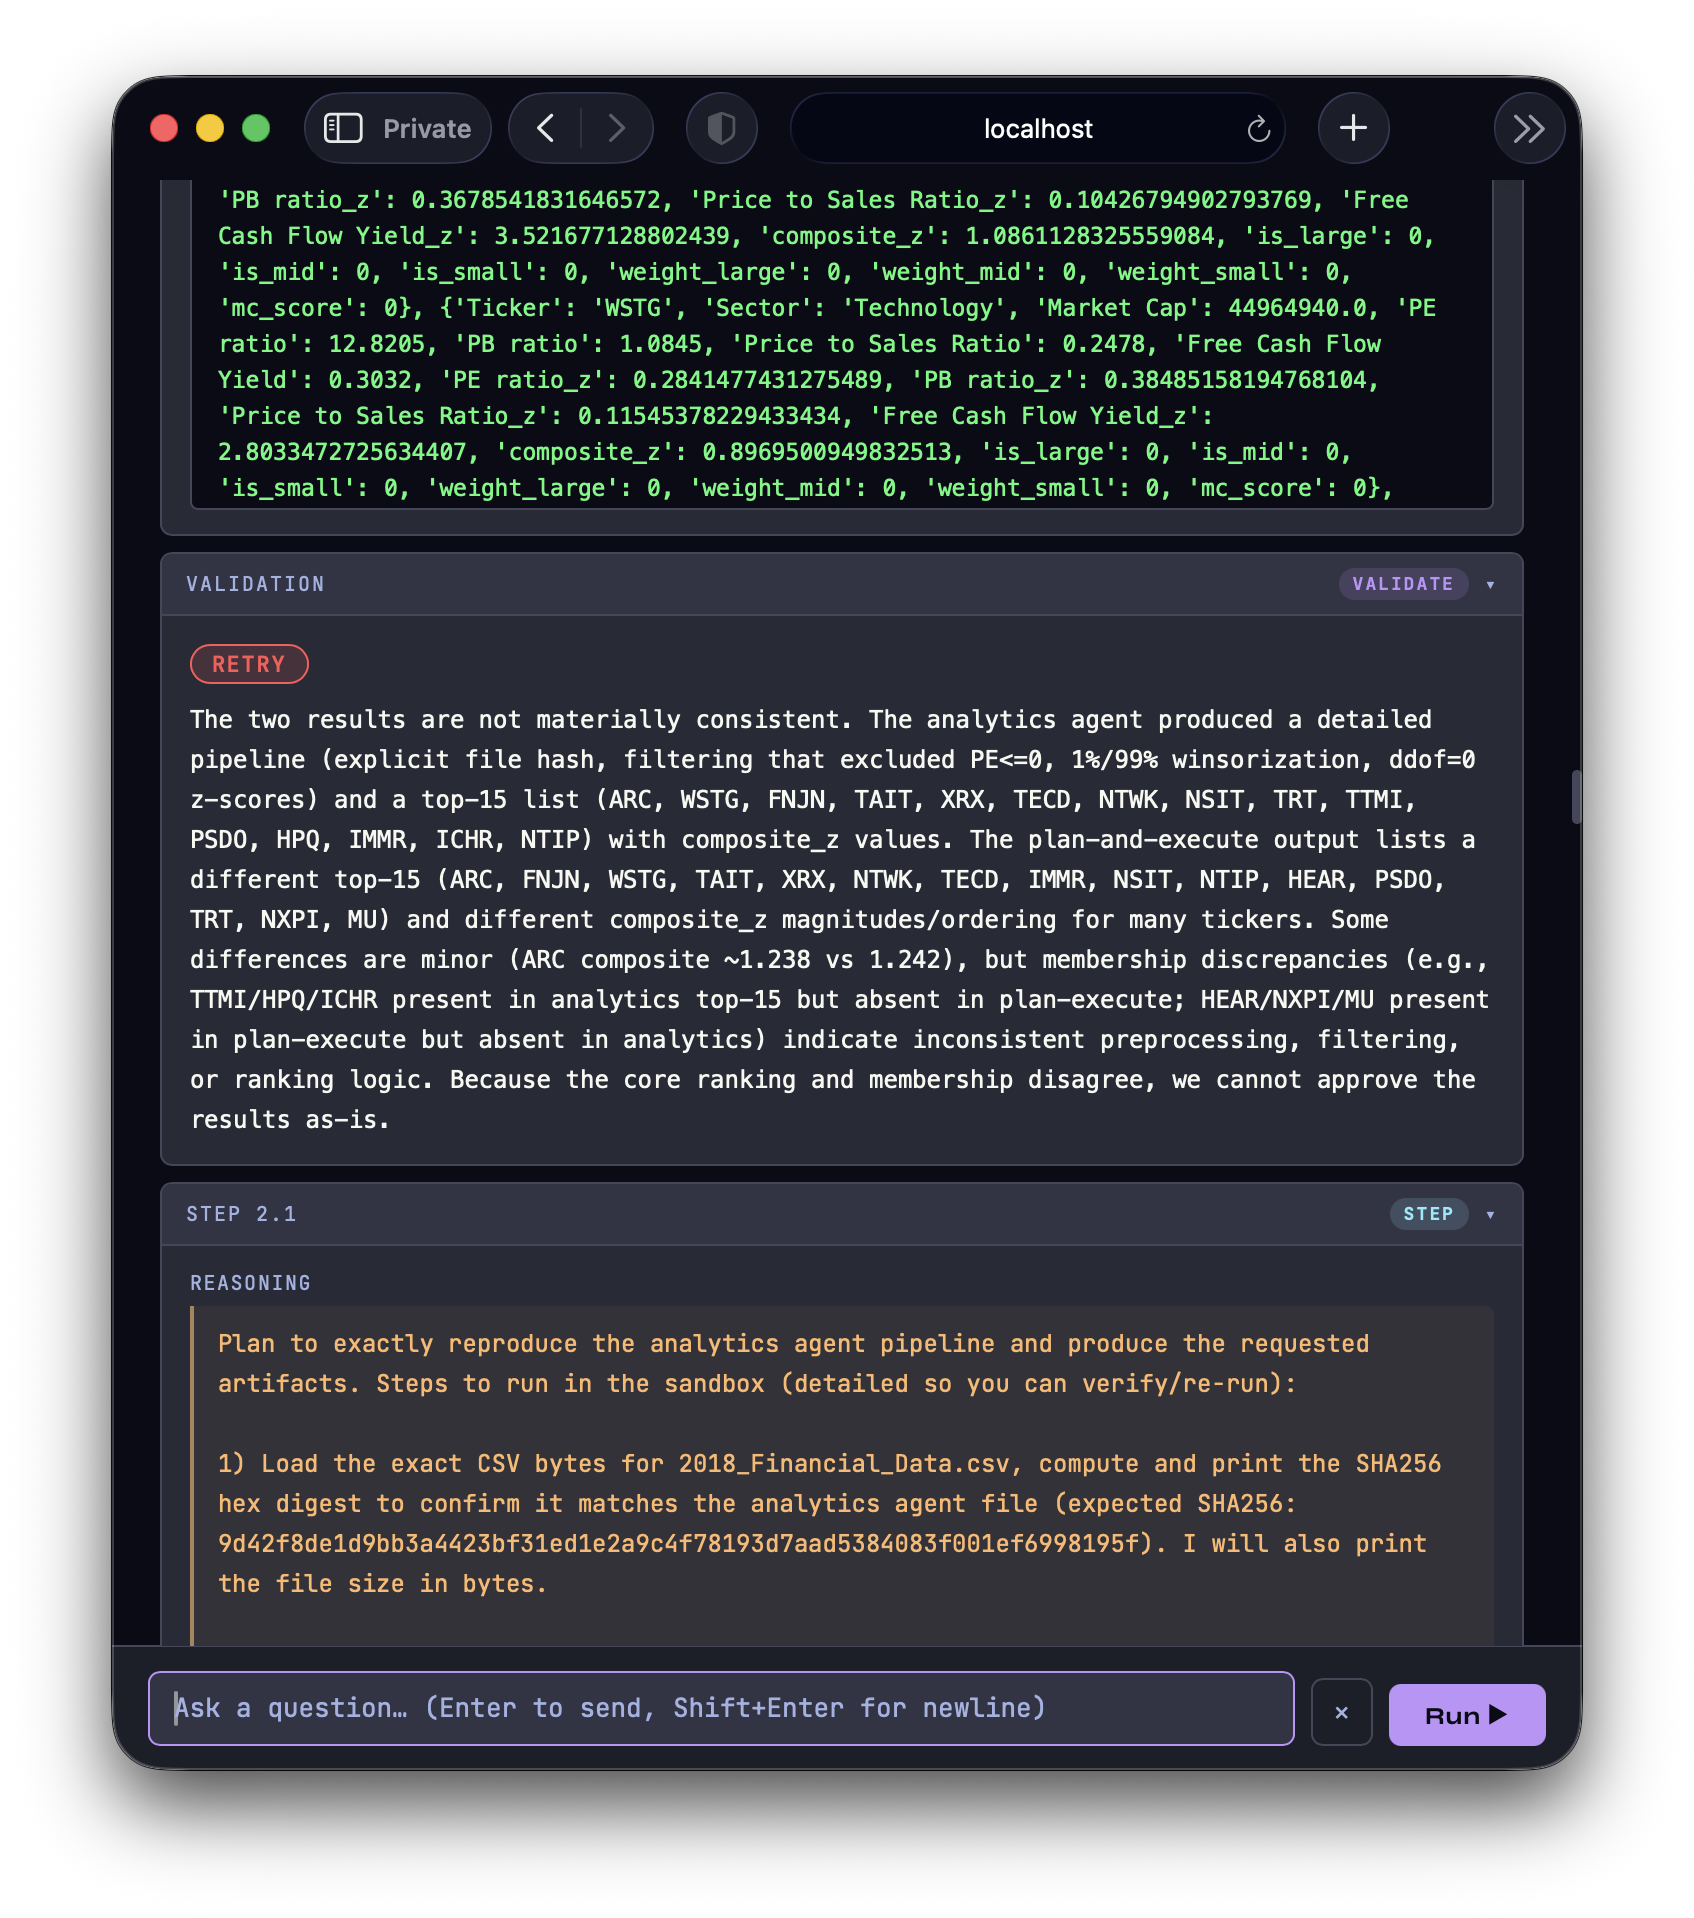
\includegraphics[width=0.4\textwidth]{graphics/ui-find-undervalued-technology-companies-from-the-dataset-produce-plots.png}
  \caption{UI Screenshot}
\end{wrapfigure}

This example demonstrates how the validator agent independently checks the analytics results, identifies inconsistencies, and requests additional analysis before allowing the workflow to continue. The example highlights the purpose of the validator as an independent reasoning component rather than a simple execution checker.

\subsect{Initial Analytics Analysis}

The analytics agent first analyzed the 2018 financial dataset to identify potentially undervalued technology companies. It:

\begin{enumerate}
  \item Loaded the 2018 dataset and filtered companies in the Technology sector.
  \item Selected valuation metrics including PE ratio, PB ratio, Price-to-Sales ratio, and Free Cash Flow Yield.
  \item Cleaned missing values and computed a composite undervaluation score.
  \item Ranked technology companies by this score.
  \item Generated supporting visualizations including scatter plots, bar charts, box plots, and correlation heatmaps.
\end{enumerate}

The analytics agent produced a top-ranked list of undervalued companies and considered the task complete.

\subsect{Validator Detects Inconsistencies}

The validator agent independently reviewed the analytics outputs and compared them against an alternative execution path. During validation, it observed that the rankings generated by different analysis runs were materially different.

The validator noted:

\begin{itemize}
  \item Different top-15 company lists.
  \item Different composite scores for the same companies.
  \item Missing agreement on preprocessing decisions.
  \item Potential inconsistencies in filtering, winsorization, and z-score calculations.
\end{itemize}

The validator therefore issued a \texttt{retry} verdict rather than approving the result. Specifically, it identified disagreements such as:

\begin{itemize}
  \item Different companies appearing in the top-ranked results.
  \item Different ranking orders.
  \item Different composite score magnitudes.
\end{itemize}

Because the numerical outputs could not be independently verified, the validator concluded that the analysis was not yet trustworthy.

\subsect{Validator Feedback Request}

Instead of simply rejecting the result, the validator generated a detailed remediation plan. It requested that the analytics workflow be rerun using a fully specified canonical pipeline.

The validator required the following information:

\begin{enumerate}
  \item Confirmation of the exact input dataset and SHA256 hash.
  \item Explicit Technology-sector filtering rules.
  \item Treatment of PE values less than or equal to zero.
  \item Counts before and after each filtering step.
  \item Exact winsorization boundaries.
  \item Exact z-score computation parameters.
  \item Directionality of each valuation metric.
  \item A reproducible top-30 output table.
  \item Source code used for the computation.
  \item Regeneration of all supporting plots.
\end{enumerate}

This feedback demonstrates that the validator reasons about correctness and reproducibility rather than merely checking whether code executed successfully.

\subsect{Retry Execution}

After receiving validator feedback, the analytics workflow was executed again with a stricter and fully documented pipeline.

The retry execution performed the following steps:

\begin{enumerate}
  \item Verified the dataset being used.
  \item Applied an exact case-insensitive filter:
    \texttt{Sector == "technology"}.
  \item Treated all PE values $\leq 0$ as missing.
  \item Dropped rows missing any required valuation metric.
  \item Applied 1\%/99\% winsorization.
  \item Computed z-scores using population standard deviation (\texttt{ddof=0}).
  \item Inverted PE, PB, and Price-to-Sales z-scores.
  \item Kept Free Cash Flow Yield positive.
  \item Computed the composite score as the average of the directional z-scores.
  \item Generated a reproducible top-30 CSV, plots, and processing script.
\end{enumerate}

The retry run also reported intermediate diagnostics such as:

\begin{itemize}
  \item Total rows: 4392
  \item Technology rows: 636
  \item Final rows after cleaning: 293
  \item Winsorization thresholds for all four metrics
  \item Means and standard deviations used in z-score calculations
\end{itemize}

\subsect{Validator Re-Validation}

Following the retry execution, the validator compared the newly generated outputs against the requested canonical specification.

The validator verified:

\begin{itemize}
  \item Matching row counts after preprocessing.
  \item Matching winsorization thresholds.
  \item Consistent z-score computation parameters.
  \item Correct handling of PE values.
  \item Availability of reproducible CSV outputs and scripts.
\end{itemize}

The retry process resolved the ambiguity that existed in the earlier analysis and produced a reproducible workflow suitable for validation.

\subsect{Key Observation}

This example illustrates the primary role of the validator agent in the HW4 architecture. The validator does not merely inspect execution success; it independently reasons about numerical correctness, reproducibility, preprocessing consistency, and completeness of analysis. When discrepancies are detected, the validator generates concrete corrective actions and forces an additional reasoning/execution cycle before the system can proceed.
